\section{Evaluation}
\label{Sec: Evaluation}

\subsection{Experimental Setup}
\label{Experimental Setup}
All experiments are conducted on a Windows 11 system with 96GB memory, one Intel® Core™ i7-14700K 3.4GHz CPU, and an NVIDIA GeForce RTX 4080 SUPER (16GB).

\textbf{Concept Drift Datasets:} 
The \pandora evaluation is conducted on five datasets: two synthetic datasets (MNIST~\cite{2017-MINIST-dataset} and Spam-Email~\cite{2010-Spam-Emali-dataset}) and three real-world datasets (APIGraph~\cite{2020-CCS-APIGraph}, Androzoo~\cite{2016-Androzoo} and BODMAS~\cite{2021-PE-malware-dataset}).
\begin{table}[h!]
	\caption{Concept Drift Datasets for Attack Evaluation}
	\label{tab: Victim Model Settings}
	\setlength{\tabcolsep}{5.8pt}
	\begin{center}
		\scalebox{1.0}{
			\begin{tabular}{cccc}
				\toprule
				\textbf{Dataset}&\textbf{Type}&\textbf{Duration}&\textbf{Size}\\
				\midrule
				APIGraph~\cite{2020-CCS-APIGraph} & Android Malware & 7 years   & 320,315\\ 
				\specialrule{0.05em}{1pt}{1pt}
				Androzoo~\cite{2016-Androzoo} & Android Malware & 6 years   & 265,740\\ 
				\specialrule{0.05em}{1pt}{1pt}
				BODMAS~\cite{2021-PE-malware-dataset}   & Windows Malware& 2 years  & 149,217 \\
				\specialrule{0.05em}{1pt}{1pt}
				MNIST~\cite{2017-MINIST-dataset}   & Image Classification& 5 cycles  & 70,000\\
				\specialrule{0.05em}{1pt}{1pt}
				SPAM~\cite{2010-Spam-Emali-dataset}     & Spam Emails & 8 cycles   & 9324     \\
				\bottomrule
		\end{tabular}}
	\end{center}
\end{table}
Detailed dataset information is presented in Table~\ref{tab: Victim Model Settings}. 
Android malware datasets span 7 years and naturally exhibit concept drift.
In contrast, non-timestamped datasets such as MNIST are typically partitioned into sub-datasets to simulate concept drift artificially.
The method for synthesizing concept drift is similar to those used in existing concept drift studies~\cite{ganguly2023online}.
%By clustering the dataset based on sample similarity and selecting a subset of similar samples for initial training, we simulate a realistic scenario where less similar data is gradually introduced in the subsequent testing data.
Synthetic dataset creation details are in Appendix~\ref{Sec: Synthetic Concept Drift Dataset Construction}.

%\begin{table}[h!]
%	\begin{center}
%		\caption{Android Concept Drift Dataset (APIGraph)} %标题
%		\label{tab: APIGraph Dataset-} %表标签
%		\renewcommand{\arraystretch}{0.8}  % 调整该表格的行距
%		\begin{tabular}{cccc} %c的个数表示表的列数
%			\toprule
%			\textbf{Year} & \textbf{Malware} & \textbf{Benign} & \textbf{Malware Family} \\
%			\midrule
%			Train-2012 & 3,061 & 27,472 & 104\\ 
%			Test-2013 (Cycle 1) & 4,854 & 43,714 & 172\\ 
%			Test-2014 (Cycle 2)& 5,809 & 52,676 & 175\\ 
%			Test-2015 (Cycle 3)& 5,508 & 51,944 & 193\\ 
%			Test-2016 (Cycle 4)& 5,324 & 50,712 & 199\\ 
%			Test-2017 (Cycle 5)& 2,465 & 24,847 & 147\\ 
%			Test-2018 (Cycle 6)& 3,783 & 38,146 & 128\\
%			\midrule
%			\textbf{Total} & \textbf{30,804} & \textbf{289,511} & \textbf{1,118}\\
%			\bottomrule
%		\end{tabular}
%	\end{center}
%\end{table}

In addition, concept drift datasets require the testing data to be partitioned according to the order of occurrence.
Following prior work~\cite{2023-Usenix-chenyizhen}, we adopt a similar setup. 
For datasets with timestamps, the APIGraph~\cite{2020-CCS-APIGraph} dataset serves as an example: data from 2012 is used for training, while data from 2013 to 2018 is used for testing, as illustrated in Table~\ref{tab: APIGraph Dataset}.
\begin{table}[h!]
	\caption{Android Concept Drift Dataset (APIGraph)}
	\label{tab: APIGraph Dataset}
	\setlength{\tabcolsep}{5.8pt}
	\begin{center}
		\scalebox{0.95}{
			\begin{tabular}{cccc}
				\toprule
				\textbf{Year}&\textbf{Malware}&\textbf{Benign}&\textbf{Malware Family}\\
				\midrule
				Train-2012 & 3,061 & 27,472 & 104\\ 
				%				\specialrule{0.05em}{1pt}{1pt}
				Test-2013 (Cycle 1) & 4,854 & 43,714 & 172\\
				%				\specialrule{0.05em}{1pt}{1pt}
				Test-2014 (Cycle 2)& 5,809 & 52,676 & 175\\ 
				%				\specialrule{0.05em}{1pt}{1pt}
				Test-2015 (Cycle 3)& 5,508 & 51,944 & 193\\
				%				\specialrule{0.05em}{1pt}{1pt}
				Test-2016 (Cycle 4)& 5,324 & 50,712 & 199\\
				%				\specialrule{0.05em}{1pt}{1pt}
				Test-2017 (Cycle 5)& 2,465 & 24,847 & 147\\
				%				\specialrule{0.05em}{1pt}{1pt}
				Test-2018 (Cycle 6)& 3,783 & 38,146 & 128\\
				\specialrule{0.05em}{1pt}{1pt}
				Total & 30,804 & 289,511 & 1,118\\
				\bottomrule
		\end{tabular}}
	\end{center}
\end{table}
In the subsequent concept drift experiments, the testing data of the APIGraph dataset is released progressively monthly.
For datasets without timestamps, the testing data is divided into multiple approximately equal-sized segments presented to the model sequentially.
The detailed information is provided in Appendix~\ref{Sec: Training and Testing Data Splits}.
Additionally, the Androzoo and APIgraph datasets represent similar scenarios and are primarily used for analyzing the impact of feature selection. Therefore, they are discussed in detail in Section~\ref{Impact of Feature Selection}.

\textbf{Victim Models:} 
The victim model’s configuration consists of two main parts: the model architecture and the sample selection strategy of active learning.
For experiments on the Android malware dataset APIGraph~\cite{2020-CCS-APIGraph}, we employ both traditional models (e.g., SVM) and deep learning models (e.g., ResNet).
The settings of sample selection strategies follow existing research on concept drift adaptation~\cite{2023-Usenix-chenyizhen,2022-SP-Trancending,2021-Usenix-CDAE,2023-survey-uncertainty-in-deep-neural-networks}.
For the other datasets (MNIST, SPAM, and BODMAS), the victim model is a multilayer perceptron consisting of five hidden layers, one output layer, and LeakyReLU activation functions.
%To prevent overfitting, the model includes batch normalization and dropout layers.
For the sample selection strategy, we use the classic confidence-based method~\cite{2023-survey-uncertainty-in-deep-neural-networks}.
%All configurations of model parameters are selected to guarantee that the victim model performs well in adapting to concept drift when no attacks are present.
%\begin{table}[h!]
%	\centering
%	\small
%	\caption{Parameters Setting of CDA-AL}
%	\label{tab: Parameter setting of active learning method}
%	%\renewcommand{\arraystretch}{1.2} % 调整单元格高度
%	\begin{tabular}{c|c c}
%		\hline
%		\textbf{Parameter} & \textbf{APIGraph} & \textbf{MNIST}\\ \hline
%		Optimizer  & SGD & ADAM\\ 
%		LR & 0.003 & 0.0004\\ 
%		Batch size & 1024 & 64\\ 
%		Loss & hi-dist-xent & triplet-mse\\ 
%		LR decay & 0.05 & - \\ 
%		Decay epochs & 10,500,10 & -\\
%		Learning epochs & 50 & 5\\ 
%		\hline
%		\textbf{Parameter} & \textbf{BODMAS} & \textbf{SPAM-Email} \\
%		\hline
%		Optimizer & AdamW & AdamW \\ 
%		LR & 0.0004 & 0.0004 \\ 
%		Batch size & 64 & 64 \\ 
%		Loss & BCE & BCE \\ 
%		LR decay & - & - \\ 
%		Decay epochs & - & - \\
%		Learning epochs & 50 & 5\\ 
%	\end{tabular}
%\end{table}
%Table~\ref{tab: Parameter setting of active learning method} summarizes the parameter settings for experiments conducted on four datasets: APIGraph~\cite{2020-CCS-APIGraph}, MNIST~\cite{2017-MINIST-dataset}, BODMAS~\cite{2021-PE-malware-dataset}, and SPAM-Email~\cite{2010-Spam-Emali-dataset}.
To prevent overfitting during model training, we adopted the same parameter settings as those used in existing concept drift adaptation methods~\cite{2023-Usenix-chenyizhen}
Additionally, we incorporated a dropout mechanism in the model trained on the BODMAS dataset, and employed early stopping strategies for models trained on the other three datasets to further mitigate overfitting. 
Moreover, as shown in Table~\ref{tab:Attack Effectiveness}, the victim models achieved an average accuracy of 97.94\% and an average F1 score of 0.88 on the testing data, indicating no signs of overfitting.
Other parameters is shown in Appendix~\ref{Sec: Model parameters}

\textbf{Attack Targets:} 
The attacker aims to continuously misclassify newly emerging concept drift samples during testing while maintaining the victim model’s overall performance.
So attack targets are selected from test samples emerging during the concept drift adaptation process.
%For example, in the malware dataset APIGraph~\cite{2020-CCS-APIGraph}, new malware samples from the testing data are chosen as attack targets.
Appendix~\ref{Sec: Attack Target List} provides detailed attack targets information.
In the real world, multiple attack targets may exist at the same concept drift cycle.
Therefore, we classify the evaluation of attack effectiveness into two types: single-target attack and multi-target attack, as shown in Section~\ref{Sec: Attack Effectiveness}.
This setup aims to understand better the impact of different attack targets settings on attack effectiveness.
It is worth noting that the multi-target attack setting simulates both a single attacker targeting multiple attack targets and multiple attackers independently targeting different targets simultaneously.

\textbf{Attack Baselines:} Given the absence of targeted poisoning attacks tailored for CDA-AL, we adapt representative adversarial concept drift poisoning attack methods to serve as baselines for comparison.

\begin{itemize}[leftmargin=0.35cm]
	\item Blind Pertubation: Apruzzese et al.~\cite{apruzzese2024adversarial} proposed a blind perturbation attack in the problem space that degrades concept drift adaptation performance in intrusion detection scenarios.
	Following this approach, we randomly select $\beta$ (labeling budget) samples from the concept drift testing data as perturbation targets and inject them into the testing data stream.
	\item Outdate Concept: Korycki et al.~\cite{2023-CCF-B-Adversarial-concept-drift-detection-under-poisoning-attacks} proposed a direction-shifting attack to mislead the concept drift adaptation process.
	Given that the direction of real-world concept drift is often unpredictable, we adopt a strategy that replays samples from the training dataset to mislead the victim model and degrade its adaptation performance.
\end{itemize}

\textbf{Metrics:} 
The effectiveness of \pandora is evaluated using the following metrics:
1) F1 Score: The harmonic mean of precision and recall, providing a balanced measure of the model’s overall performance on the testing data.
2) Attack Effectiveness: Effectiveness is assessed via the attack success rate (ASR), where success is defined as the victim model misclassifying the specific attack target.
Additionally, since attack targets may already be misclassified during the early stages of concept drift, we adopt a more stringent criterion for measuring attack success.
Only when the \pandora prolongs the duration of the attack target’s misclassification will the attack be regarded as successful, as defined in Equation~\ref{Attack Persistence}.
$N$ denotes the \pandora testing cycle length for the attack target $\bm{\mathrm{x}}_{tar}$. 
Function $Judge()$ compares the ground truth label $y_{tar}$ of $\bm{\mathrm{x}}_{tar}$ with the victim model’s predicted label $\overline{y}_{tar}$. 
A mismatch between them during the testing cycle indicates a successful attack.
Since all experiments in this study require running multiple testing cycles, the testing phase incurs significant time overhead.
Therefore, in subsequent experimental evaluations, the testing cycle extension is set to 1 for all cases except for dedicated attack persistence tests, which utilize a full 100\% testing cycle extension.
All reported performance metrics are averaged over five attack runs per target.
A small standard deviation reflects the consistency and stability of the results.
\begin{align}
	Judge(y_{tar}, & \overline{y}_{tar},n) =
	\begin{cases} 
		0,y_{tar}=\overline{y}_{tar} \, at \,\, $n$, \\
		1,y_{tar} \neq \overline{y}_{tar} \, at \,\, $n$.
	\end{cases}  \\
	ASR(y_{tar},& \overline{y}_{tar},n,N)  = \frac {\sum_{n=1}^{N}Judge(y_{tar}, \overline{y}_{tar},n)}{N}
	\label{Attack Persistence}
\end{align}

\subsection{Attack Effectiveness}
\label{Sec: Attack Effectiveness}
The effectiveness of \pandora is evaluated on five datasets across different domains.
Due to its long time span and real-world dataset, the APIGraph dataset~\cite{2020-CCS-APIGraph} is utilized for both single-target and multi-target attacks.
The manually synthesized concept drift datasets (MNIST~\cite{2017-MINIST-dataset} and SPAM~\cite{2010-Spam-Emali-dataset}), as well as the BODMAS malware concept drift dataset~\cite{2021-PE-malware-dataset}, contain a limited number of attack targets and span a short time period.
Therefore, they are utilized to evaluate multi-target attack scenarios.

\subsubsection{Single-Target Attack} 
\label{Sec: Single Attack Targets}
We assess the effectiveness of the \pandora with a simple attack target on the APIGraph~\cite{2020-CCS-APIGraph} dataset.
The evaluation of attack effectiveness involves more than 300 attack targets.
Appendix~\ref{Sec: Attack Target List} provides detailed information on the attack targets.

\begin{table}[h!]
	\caption{Effectiveness of Different Attack Strategies}
	\label{tab: attack-baselines}
	\setlength{\tabcolsep}{5.8pt}
	\begin{center}
		\scalebox{1.0}{
			\begin{tabular}{ccccc}
				\toprule
				\textbf{Attack Strategies}&\textbf{F1 Score} &\textbf{ACC} &\textbf{ASR (\%)} \\
				\midrule
				Blind Pertubation~\cite{apruzzese2024adversarial} & 0.92 & 0.98 & 38.16\% \\ 
				\specialrule{0.05em}{1pt}{1pt}
				Outdate Concept~\cite{2023-CCF-B-Adversarial-concept-drift-detection-under-poisoning-attacks} & 0.92 & 0.98 & 34.31\%\\
				\specialrule{0.05em}{1pt}{1pt}
				%				Noise Concept Drift~\cite{2023-CCF-B-Adversarial-concept-drift-detection-under-poisoning-attacks} & 0.92  & 0.92 &81.68\% \\ 
				%				\specialrule{0.05em}{1pt}{1pt}
				\pandora (Our Attack) & 0.90  & 0.98 & 89.22\% \\ 
				\bottomrule
		\end{tabular}}
	\end{center}
\end{table}
We first apply problem-space adversarial perturbation to generate poisoned samples.
Subsequently, by employing concept drift direction misguidance, we enhance the poisoning process for attack targets where the problem-space perturbation strategy proves ineffective.
This setup allows us to illustrate better how perturbations in the feature space can enhance the effectiveness of problem-space perturbations.
To efficiently demonstrate the effectiveness of \pandora, we compare it with two existing adversarial concept drift poisoning attack methods, as shown in Table~\ref{tab: attack-baselines}.
The \pandora demonstrates high effectiveness, achieving an average ASR of 89.22\%.
This implies that the \pandora can extend the misclassification duration of most attack targets during the process of CDA-AL.
In addition, compared to existing attack methods, \pandora significantly improves the attack success rate, with an average increase of 52.99\%.
Moreover, the overall performance of the victim model remains stable, with an F1 score of 0.9 and an accuracy of 98\%.

\begin{table}[ht]
	\caption{Concept Drift Datasets for Attack Evaluation}
	\label{tab:Attack Effectiveness}
	\setlength{\tabcolsep}{5.8pt}
	\begin{center}
		\scalebox{1.0}{
			\begin{tabular}{cccc}
				\toprule
				\textbf{Attack Target}&\textbf{ASR(\%)}&\textbf{F1 score}&\textbf{ACC(\%)}\\
				\midrule
				Mecor (Trojan-Spy) & 100\%  & 0.85 (-0.07) & 97.49(-1.07)\\ 
				\specialrule{0.05em}{1pt}{1pt}
				Mobidash (Adware) & 100\%  & 0.90 (-0.02) & 98.28 (-0.28) \\
				\specialrule{0.05em}{1pt}{1pt}
				Svpeng (Banking Trojan) & 80.00\%  & 0.90 (-0.02) & 98.26 (-0.30)\\
				\specialrule{0.05em}{1pt}{1pt}
				Smforw (Trojan-Spy) & 100\%  & 0.81 (-0.11) & 96.80 (-1.76)\\
				\specialrule{0.05em}{1pt}{1pt}
				Fobus (Data Stealing) & 42.86\%   & 0.88 (-0.04) & 97.84 (-0.72)\\
				\specialrule{0.05em}{1pt}{1pt}
				Adflex (Adware) & 100\%  & 0.90 (-0.02) & 98.26 (-0.30)\\
				\specialrule{0.05em}{1pt}{1pt}
				Vnapstore (Unknown) & 100\%   & 0.85 (-0.07) & 97.41 (-1.15)\\
				\specialrule{0.05em}{1pt}{1pt}
				Clicks (Trojan-Spy) & 60\%   & 0.90 (-0.02) & 98.40 (-0.16)\\
				\specialrule{0.05em}{1pt}{1pt}
				Mogap (Trojan-Spy) & 100\%   & 0.90 (-0.02) & 98.24 (-0.32)\\
				\specialrule{0.05em}{1pt}{1pt}
				Congur (Trojan-Spy) & 87.50\%   & 0.91 (-0.01) & 98.40 (-0.16)\\
				\bottomrule
		\end{tabular}}
		\begin{tablenotes}
			\footnotesize
			\item The proportion of poisoned samples in the monthly testing data averages less than 0.06, demonstrating a high level of attack stealth.
		\end{tablenotes}
	\end{center}
\end{table}
In Table~\ref{tab:Attack Effectiveness}, we present the top 10 malware families of attack targets with the most significant number of samples, along with their attack success rates and the performance metrics of the victim model.
In addition to the fact that 60\% of the attack targets families achieve an ASR of 100\%, we focus on whether the impact of the \pandora on the victim model’s performance is sufficiently minimal to enhance its attack stealth.
We observe that the F1 fluctuations remain within 0.2, while the ACC stays above 95\%.
The model’s average TNR under \pandora reaches 99\%, ensuring minimal false alarms.
Based on the above data, it can be concluded that the poisoned sample generation strategy based on problem-space adversarial perturbation effectively prevents the victim model from learning the attack targets while maintaining its overall performance during the CDA-AL. 
We further measured the problem-space perturbation time for programs of varying sizes. Experiments on several widely-used programs show that the average perturbation time remains under 100 seconds, as shown in Table~\ref{tab: APK obfdxuscation time}.
In addition, the process can be supported by a range of well-established tools, highlighting the cost-effectiveness of problem-space perturbation.
\begin{table}[h!]
	\centering
	\small
	\renewcommand{\arraystretch}{0.8}
	\caption{APK obfuscation Time}
	%\renewcommand{\arraystretch}{0.8}  % 调整该表格的行距
	\label{tab: APK obfdxuscation time}
	\begin{tabular}{c|c|c}
		\toprule
		\textbf{APK} & \textbf{Size (MB)} & \textbf{Obfuscation time} \\
		\midrule
		JD & 97.59 & 54.95s \\
		Taobao & 57.03 & 78.98s \\
		Little Red Book & 162.99 & 178.68s \\
		Google & 315.67 & 93.32s \\
		Wang VPN & 45.51 & 14.91s \\
		WeChat & 264.04 & 136.76s \\
		\midrule
		\textbf{Average} & 199.72 & 90.72s \\
		\bottomrule
	\end{tabular}
\end{table}
%\begin{table}[h!]
%	\caption{Time overhead of problem-space perturbation}
%	\label{tab: APK obfuscation time}
%	\setlength{\tabcolsep}{5.8pt}
%	\begin{center}
%		\scalebox{1.0}{
%			\begin{tabular}{ccc}
%				\toprule
%				\textbf{APK}&\textbf{Size (MB)}&\textbf{Time Overhead}\\
%				\midrule
%				JD & 97.59 & 54.95s \\
%				\specialrule{0.05em}{1pt}{1pt}
%				Taobao & 57.03 & 78.98s \\
%				\specialrule{0.05em}{1pt}{1pt}
%				Little Red Book & 162.99 & 178.68s \\
%				\specialrule{0.05em}{1pt}{1pt}
%				Google & 315.67 & 93.32s \\
%				\specialrule{0.05em}{1pt}{1pt}
%				Wang VPN & 45.51 & 14.91s \\
%				\specialrule{0.05em}{1pt}{1pt}
%				WeChat & 264.04 & 136.76s \\
%				\bottomrule
%		\end{tabular}}
%	\end{center}
%\end{table}

Since the victim model is continuously updated during the concept drift adaptation process, it is necessary to test whether \pandora's effectiveness persists over time.
To ensure a fair comparison across different attack targets, we standardized the testing period.
The testing cycle for each attack target is extended to 200\% of the original duration of misclassification, based on the initial misclassification results (as shown in Appendix~\ref{Sec: Attack Target Initial Survival Time (APIGraph)}).
For instance, if the attack target is detected as malicious in the fourth month after its first appearance, we conduct an 8-month attack effectiveness test.
The attack is considered successful only if the \pandora extends the target’s misclassification duration for the whole 8 months.
To illustrate attack persistence trends, we selected malware samples per month from January 2013 to December 2018 as attack targets.
During the six-year concept drift adaptation process, an average Attack Success Rate (ASR) of 87.33\% was achieved, as shown in Figure~\ref{fig:Attack Persistence-APIGraph}.
Therefore, it is evident that the \pandora ensures the attack targets remains persistently misclassified throughout the long-term concept drift adaptation process of the victim model.
This poses a significant threat to the field of concept drift adaptation, as the core objective of concept drift adaptation methods is to minimize the duration of misclassification.
\begin{figure}[h!]
	\centering
	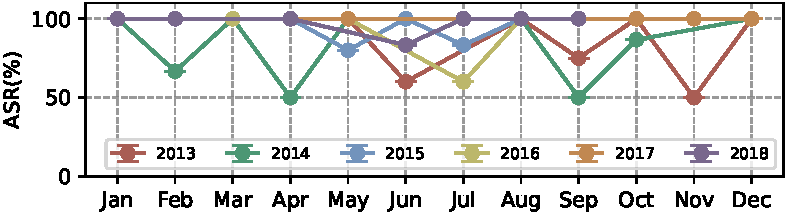
\includegraphics[width=\linewidth,keepaspectratio]{Graph/Evaluation/Figure9-update.pdf}
	\caption{Attack Persistence over 6 years }
	\label{fig:Attack Persistence-APIGraph}
\end{figure}

The effectiveness of the \pandora using the problem-space adversarial perturbation in poisoned sample generation has already been validated. 
Next, we evaluate the effectiveness of the concept drift direction misguidance.
We selected 138 families with less than six months of survival for comparative analysis. 
We divided the attack targets into five groups based on the duration of the attack test.
The results of the attack’s effectiveness are presented in Figure~\ref{fig:feature-space perturbation strategy}.
\begin{figure}[h!]
	\centering
	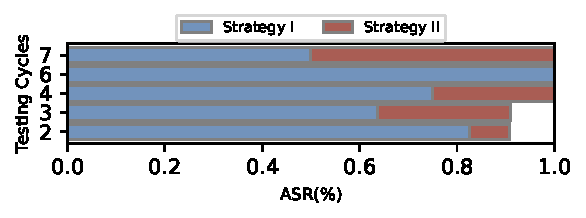
\includegraphics[width=\linewidth,keepaspectratio]{Graph/Evaluation/Figure26.pdf}
	\caption{Feature-space perturbation strategy}
	\label{fig:feature-space perturbation strategy}
\end{figure}
After introducing the concept drift misguidance based on the shapley additive explanations, the attack success rate improved for most targets, reaching an average of 91.3\%.
This represents a 10.9\% increase compared to the previous attack success rate achieved with the problem-space perturbation strategy.
The increase in ASR is due to the attacker’s ability to generate poisoned samples with higher uncertainty than those produced using the problem-space adversarial perturbation strategy.
After applying concept drift misguidance, the average uncertainty ranking of the poisoned samples increased by 66.2\%.
This further demonstrates the complementary roles of the two modules in the generation of poisoned samples by \pandora.

In addition, since computational cost is a primary concern in machine learning scenarios, the attacker’s model was weakened to reduce computational overhead.
Specifically, we weaken the model by reducing the number of neural network layers in the encoder or classifier.
Following state-of-the-art Android malware concept drift adaptation methods~\cite{2023-Usenix-chenyizhen}, which employ an encoder and classifier, we tested four weakened settings based on the victim model, as shown in Figure~\ref{fig:Attack-effectiveness-model-heterogeneity}.
ENC denotes the encoder, CAL represents the classifier, and W indicates a decrease in the model’s capacity, reflected in a reduction of model parameters.

\begin{figure}[h!]
	\centering
	\includegraphics[width=\linewidth,keepaspectratio]{Graph/Evaluation/Figure10_1.pdf}
	\caption{Attack Effectiveness under Weakened Capabilities}
	\label{fig:Attack-effectiveness-model-heterogeneity}
\end{figure}
\begin{figure*}[t]
	\centering
	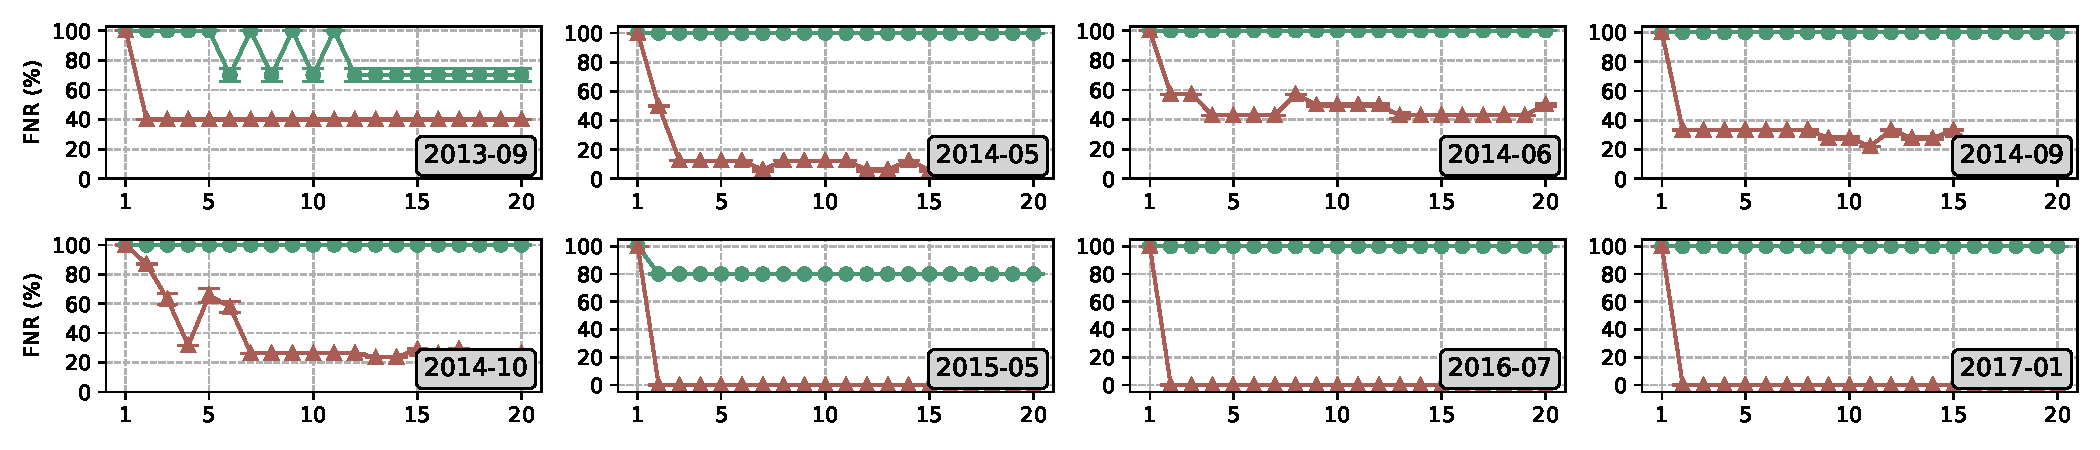
\includegraphics[width=\linewidth,keepaspectratio]{Graph/Evaluation/api_multi_attackers_fnr_1-up.pdf}
	\caption{Attack Effectiveness with Multi-Target Attack (6 year Attack Testing)}
	\label{fig: Attack Effectiveness with Multi-Target Attack}
\end{figure*}

Previous studies have shown that when the attacker’s capabilities are limited, the effectiveness of poisoning attacks decreases~\cite{2022-ACM-Computing-Survey-Threats-to-training}.
However, \pandora mitigates this issue, achieving an average attack success rate of 81.17\% with limited attacker capabilities, as shown in Figure~\ref{fig:Attack-effectiveness-model-heterogeneity}. 
We also found that weakening the encoder reduces the attack success rate by nearly 10\%, which is more significant than weakening the classifier.  
This indicates that the encoder part of the surrogate model plays a crucial role in approximating the capabilities of the victim model.
Additionally, we found that weakening both the encoder and the classifier in the attacker’s surrogate model does not result in the lowest attack success rate.
Under this configuration, the attack success rate is even higher than that of the setup where only the classifier is weakened, at 86\% compared to 83\%.
This phenomenon contradicts the expectation that attackers must invest more computational resources to achieve a higher attack success rate.
By analyzing the set of attack targets under different configurations, we found that when the surrogate model is weakened, its selection of attack targets is significantly biased.
In the synchronized weakening setting, only 55\% of the attack targets remain compared to the control group, highlighting the need to assess attack effectiveness under constrained attacker capabilities using ASR and the number of attack targets.
To address this issue, we define the Number of Successful Attack Targets (NSAT) and the Relative Attack Success Rate (RASR), which represents the ratio of successfully attacked targets in the weakened attacker’s setup to those in the control group, as shown in Equation~\ref{attack seed formula 1}.
\begin{equation}
	\begin{aligned}
		RASR = \small NSAT_{weak}/\small NSAT_{control}
	\end{aligned}
	\label{attack seed formula 1}
\end{equation}
As model capability weakens, RASR declines, with the weakest setup showing a 43.18\% drop.
While a reduced scope of attack targets weakens the attacker’s capabilities, the relative attack success rate increases, posing a significant threat to concept drift adaptation by enhancing resource utilization efficiency even under constrained conditions.

\subsubsection{Multi-Target (Attacker) Attack} 
\label{Sec: Multi Attack Targets}
As described in Section~\ref{Experimental Setup}, the multi-targets setting simulates two practical scenarios: (1) a single attacker launching attacks against multiple targets, and (2) multiple attackers independently targeting different targets.
For clarity and ease of analysis, we adopt the first scenario, where a single attacker conducts multi-target attacks, as the basis for the following discussion.
Multiple attack targets may emerge within the same concept drift cycle in real-world scenarios. 
Therefore, \pandora also supports a multi-target attack mode.
In the multi-target attack setting, the attacker performs \pandora on multiple attack targets simultaneously.
To evaluate the effectiveness of the \pandora in a multi-target setting, we selected 8 months with different attack targets for testing, covering a 6-year evaluation period, as illustrated in Figure~\ref{fig: Attack Effectiveness with Multi-Target Attack}.
For each multi-target setting, we conducted a 20-month attack test.
Detailed information on the settings can be found in Appendix~\ref{Sec: Attack Target List}.
The multi-target attack achieved an average success rate of 97.5\% across different testing times, demonstrating its effectiveness in executing the \pandora on multiple targets.
During the 80-month attack test, only the attack success rate in May 2015 was not 100\%, although it still maintained an effective success rate of 80\%.
The high attack success rate in a multi-target setting is due to the coverage effect of labeling budget consumption across different attack targets.
When multiple attack targets are present, once the labeling budget for the most uncertain attack target is exhausted, the labeling budget for the other attack targets is also concurrently depleted.
Consequently, the \pandora incurs a low cost, as a single attack benefits multiple targets simultaneously.

Then we discuss the scenario where multiple distinct attackers simultaneously target different attack targets.
In terms of attack effectiveness, the success rate in the multi-attacker setting is consistent with that in the single attacker setting with multiple attack targets.
This is because, as previously analyzed, the poisoned samples generated for different attack targets do not interfere with one another.
In fact, poisoned samples crafted for attack targets with the highest uncertainty can even facilitate the misclassification of other attack targets.
Furthermore, we observe that when attack effects are mutually beneficial, attackers tend to cooperate, thereby reducing the overall attack cost. Specifically, multiple attackers can identify the attack target with the highest uncertainty and use it as a common target, allowing them to share the costs involved in poisoned sample generation.
%接下来我们讨论多个不同攻击者对不同攻击目标同时进行攻击的情况。
%在攻击效果方面,多攻击者的攻击成功率与单一攻击者攻击多个目标设置下的攻击成功率是一样的。
%因为如上述分析所示,针对不同攻击目标生成的投毒样本彼此之间不会产生相互干扰,反而是具有最高不确定性的攻击目标生成的投毒样本可以辅助其他攻击目标成功实现误分类的攻击效果。
%并且我们发现在攻击效果可以彼此收益的情况下,攻击者之间会倾向于相互合作,进而降低整体的攻击成本。
%因为多个不同的攻击者可以选出攻击目标中不确定性最高的样本作为群体攻击目标,进而分摊投毒样本生成过程中的各种开销。
\begin{table}[h!]
	\caption{Multi-Target Attack across Four Ddatasets}
	\label{tab: asz }
	\setlength{\tabcolsep}{5.8pt}
	\begin{center}
		\scalebox{1.0}{
			\begin{tabular}{ccccc}
				\toprule
				\textbf{Datasets}&\textbf{Targets}&\textbf{F1-Testing} &\textbf{F1-Validation} &\textbf{ASR (\%)} \\
				\midrule
				APIGraph & 331  &  0.76\textsubscript{\textcolor{black}{-0.15}} & 0.99 & 92.92\% \\ 
				\specialrule{0.05em}{1pt}{1pt}
				MNIST & 1,398  & 0.78\textsubscript{\textcolor{black}{-0.12}} & 0.99 & 79.98\%\\
				\specialrule{0.05em}{1pt}{1pt}
				BODMAS & 222  &  0.92\textsubscript{\textcolor{black}{-0.06}}& 0.92 &80.63\% \\ 
				\specialrule{0.05em}{1pt}{1pt}
				SPAM & 168  &  0.91\textsubscript{\textcolor{black}{-0.07}} & 0.99 &74.40\% \\ 
				\bottomrule
		\end{tabular}}
	\end{center}
\end{table}

In certain special cases, the attacker may need to target all attack targets simultaneously.
This represents a special scenario within multi-target attacks.
Therefore, we tested the effectiveness of \pandora on all attack targets at different concept drift time points.
The average attack success rate reaches 81.98\% (as shown in Table~\ref{tab: asz }), with a notably high success rate of 92.92\% achieved on the real-world concept drift dataset, APIGraph.  
Moreover, we observe that the victim models maintain high F1 scores on the initial validation set under attack across different datasets, with an average of 0.99.
This demonstrates that our method preserves the victim model’s previously learned knowledge, even when targeting all attack targets, thereby highlighting the stealth of the proposed attack.
The impact on test performance (F1-Testing) varies across datasets, reflecting how limited access to new samples can hinder the model’s adaptation to concept drift.
The performance degradation on the BODMAS and SPAM datasets is relatively minor, with average F1-score drops of less than 0.07, indicating a lower intensity of concept drift in these scenarios.
In contrast, the APIGraph and MNIST datasets exhibit more substantial performance changes, with average F1-score drops of around 0.14.
This suggests stronger concept drift and a higher reliance on the victim model for effective learning from drifted samples.
Nevertheless, \pandora stealth remains unaffected in both cases, as the testing data is unlabeled, and the victim model cannot promptly detect its performance degradation.

\subsection{Attack Influencing Factors}
\label{Sec: Attack Influencing Factors}

We have demonstrated the effectiveness of \pandora.
To further investigate how real-world conditions affect attack performance, we analyze the factors influencing \pandora using a real-world Android malware dataset (APIGraph~\cite{2020-CCS-APIGraph}) spanning seven years.

\subsubsection{Impact of Different CDA-AL Strategies}
Existing concept drift adaptation strategies in sensitive domains~\cite{2023-Usenix-chenyizhen,2022-SP-Trancending,2021-Usenix-CDAE} can be broadly categorized into four types. 
In addition to the uncertainty-based strategies discussed in Section~\ref{Sec: Concept Drift Adaptation}, the remaining approaches fall into three categories. 
To ensure the generality of our findings, we evaluate the effectiveness of \pandora across all these representative adaptation strategies.

\begin{itemize}[leftmargin=0.35cm]

\item CADE~\cite{2021-Usenix-CDAE} trains an encoder with labeled data to learn compressed input representations. 
It uses a distance function to identify concept drift samples that deviate from the training data.
\begin{equation}
	\begin{aligned}
		d_{i} = ||\bm{\mathrm{z}}_{i}-\bm{\mathrm{zc}}_{i}||_{2} \\
	\end{aligned}
	\label{CADE}
\end{equation}
Specifically, $\bm{\mathrm{z}}_{i}$ represents the latent space embedding of the sample $\bm{\mathrm{x}}_{i}$ obtained from the encoder. 
A sample is a concept drift instance if its distance $d_{i}$ to the nearest training sample in the encoder’s latent space exceeds a predefined threshold.
\item TRANS~\cite{2022-SP-Trancending}
applies conformal prediction~\cite{2005-high-cite-Algorithmic-learning-in-a-random-world} to concept drift adaptation.
It calculates a testing sample’s non-conformity score, credibility (proportion of calibration samples with higher scores), and confidence (1 minus the opposite label’s credibility). 
Low scores indicate potential drift.
\item HCL~\cite{2023-Usenix-chenyizhen}
proposes the latest concept drift adaptation strategy, combining an encoder and classifier. 
Its training loss $\mathcal{L}(\bm{\mathrm{x}}_{i})$ integrates hierarchical contrast loss $\mathcal{L}_{hc}(\bm{\mathrm{x}}_{i})$ and classification loss $\mathcal{L}_{ce}(\bm{\mathrm{x}}_{i})$.
\begin{equation}
	\begin{aligned}
		\mathcal{L}(\bm{\mathrm{x}}_{i}) = \mathcal{L}_{hc}(\bm{\mathrm{x}}_{i}) + \mathcal{L}_{ce}(\bm{\mathrm{x}}_{i}) \\
	\end{aligned}
	\label{CADE}
\end{equation}
Samples with higher loss values are more likely to be affected by concept drift, as different samples incur different loss levels during inference.

\end{itemize}
%The evaluation includes both traditional model uncertainty approaches and concept drift adaptation strategies that leverage advanced machine learning techniques, such as contrastive learning.
%As shown in Figure~\ref{fig:Attack-effectiveness-Concept-Drift-Strategy}, the experimental results demonstrate that our attack consistently achieves an attack success rate exceeding 80\% across four various concept drift adaptation strategies.
%Furthermore, during the attack process, the performance metrics of the primary task remain stable, with the F1 consistently exceeding 0.88 across all strategies.
%Notably, the ASR reaches 92.77\% when targeting the currently optimal concept drift adaptation method (HCL).
%The primary reason \pandora achieves the highest attack success rate on HCL is that HCL selects concept drift samples based on their loss function values, making the constructed poisoned samples significantly impact the retraining process of the victim model.
%As a result, ensuring the security of concept drift adaptation methods has become an urgent challenge requiring immediate attention.
% Version
%The evaluation includes traditional uncertainty-based approaches and advanced concept drift adaptation strategies, such as contrastive learning.
%As shown in Figure~\ref{fig:Attack-effectiveness-Concept-Drift-Strategy}, \pandora achieves an ASR exceeding 80\% across all four strategies while maintaining stable primary task performance, with F1 consistently above 0.88.
%Notably, \pandora achieves a 92.77\% ASR against the optimal concept drift adaptation method (HCL).
\begin{figure}[h!]
	\centering
	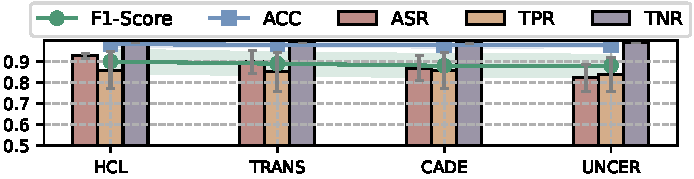
\includegraphics[width=\linewidth,keepaspectratio]{Graph/Evaluation/Figure13.pdf}
	\caption{Different Concept Drift Adaptation Strategies}
	\label{fig:Attack-effectiveness-Concept-Drift-Strategy}
\end{figure}
The evaluation covers traditional uncertainty-based methods and advanced concept drift strategies like contrastive learning.
As shown in Figure~\ref{fig:Attack-effectiveness-Concept-Drift-Strategy}, \pandora achieves over 80\% ASR across all four strategies while maintaining F1 scores above 0.88.
\pandora attains a 92.77\% ASR against the latest adaptation method (HCL).
%These results highlight the urgent need to address security challenges in concept drift adaptation methods.

%\begin{figure}[h!]
%	%\vspace{-0.8em}
%	\centering
%	\subfloat[Different Strategies]{
%		\label{fig11-1}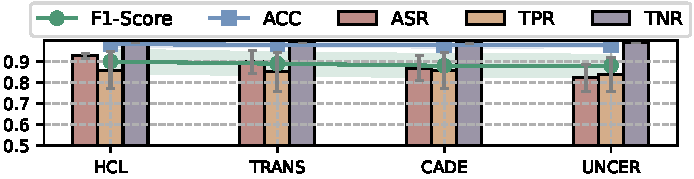
\includegraphics[width=4.25cm, height=2.9cm]{Graph/Evaluation/Figure13.pdf}
%	}
%	\subfloat[Labeling Budget]{
%		\label{fig11-2}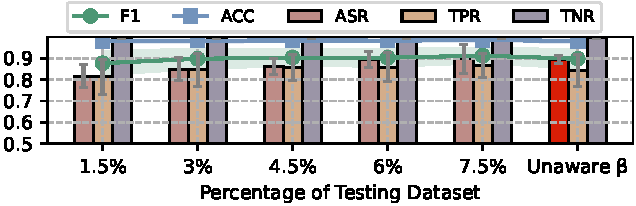
\includegraphics[width=4.25cm, height=2.9cm]{Graph/Evaluation/Figure14_3.pdf}
%	}
%	\caption{xxxxxxxxxxxxx.} 
%	\label{fig111}
%	%\vspace{-1em}
%\end{figure}

\subsubsection{Impact of Labeling Budget}
\label{Sec: Attack Effectiveness under Different Label budget}
The labeling budget represents the cost of manual labeling and is one of the most valuable resources in CDA-AL.
We evaluated the attack effectiveness under six different labeling budget settings.
Each labeling budget setting represents its proportion of the testing data, following the settings of existing studies~\cite{2023-Usenix-chenyizhen}.
The first five labeling budget settings assume the attacker knows the victim model’s labeling budget.
In contrast, the last setting assumes the attacker cannot access the victim model’s labeling budget.
When the attacker is unaware of the labeling budget settings, poisoned samples are generated based on the maximum computational capacity of the attacker. 
In this experiment, we set the attacker’s capacity four times the potential labeling budget computation capacity.
\begin{figure}[h!]
	\centering
	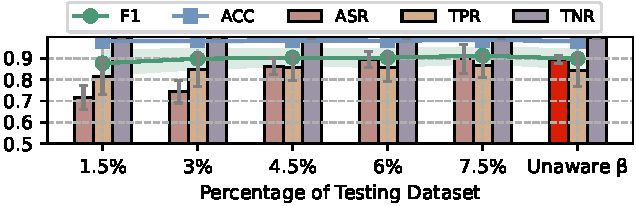
\includegraphics[width=\linewidth,keepaspectratio]{Graph/Evaluation/Figure14_4.pdf}
	\caption{\pandora Under Different Labeling Budget}
	\label{fig:Attack-effectiveness-Label-Budget}
\end{figure}
As shown in Figure~\ref{fig:Attack-effectiveness-Label-Budget}, \pandora remains effective across budgets, with an average attack success rate of 85.10\%.
Even without access to the victim model’s labeling budget, the attacker can still achieve a high attack success rate by leveraging the maximum available resources, reaching 89.33\%.
The high attack success rate, even without access to detailed labeling budget information, is due to the significantly lower cost of poisoning attacks than the victim’s concept drift adaptation cost, which is primarily driven by labeling expenses.
Thus, the attacker can generate as many poisoned samples as possible to consume the victim model’s labeling budget.
This strategy is inspired by DDoS~\cite{mirkovic2004taxonomy} attacks, where the attacker maximizes attack traffic without knowing the victim’s total resources to achieve the attack objective.
Moreover, even if the scale of poisoned samples in the \pandora attack exceeds the labeling budget, it is unlikely to raise suspicion.
This is because the poisoned samples are injected into the unlabeled testing data stream during each concept drift cycle, and the volume of this stream is substantially larger than the victim model’s monthly labeling budget.
As a result, \pandora exhibits strong stealth. 
Furthermore, it is extremely difficult for the victim model to detect poisoned samples within the testing data stream due to the massive volume of incoming data, which makes full inspection infeasible.

%In our setup, the label budget reflects a victim model’s real-world capabilities.\footnote{According to Kaspersky’s 2023 statistics~\cite{Kaspersky-Android-Malware-Threat-Statistics}, the total number of Android malware samples for the year reached 1.12 million. Using the commonly assumed 9:1 ratio of benign to malicious samples, the total number of benign and newly detected malicious samples per month is estimated to be 11.2 million.}
%The maximum budget of 300 samples represents approximately 9\% of the monthly test data, which is equivalent to the manual analysis of 83,761 samples each month in real-world scenarios.
%An estimated cost of 22 USD per sample (obtained through interviews with security vendors) translates to 1.84 million USD per month, representing a substantial financial burden for security companies.

%\subsubsection{Impact of Data Collection Capability}
%In multi-target attacks, there is a special case where the attack target consists of all the test data.
%In this case, the attacker’s poisoning seed samples need to be the highest uncertainty samples from the test dataset, making data collection capability crucial to its effectiveness.
%So we conducted attack experiments with five settings on four datasets.
%\pandora relies on identifying high-uncertainty attack seeds to generate poisoned samples.
%The uncertainty of these seeds is influenced by the attacker’s data collection capabilities, affecting the overall attack effectiveness.
%Tests were conducted across four datasets under different data collection capacities to analyze their effects on attack performance, as illustrated in Figure~\ref{fig:Impact of Data Collection Ability}.
%\begin{figure}[t]
%	\centering
%	\includegraphics[width=\linewidth,keepaspectratio]{Graph/Evaluation/figure17-v3.pdf}
%	\caption{Impact of Data Collection Ability}
%	\label{fig:Impact of Data Collection Ability}
%\end{figure}
%No clear correlation was observed between reduced data collection capability and diminished attack effectiveness.
%Across all four datasets, reduced data collection sometimes improved attack performance. 
%For instance, in the MNIST dataset, attacks with 90\% data collection capability outperformed those with 100\% capability in over 80\% of the attack test cycles.
%Similarly, in the APIGraph~\cite{2020-CCS-APIGraph} dataset, 50\% capability occasionally surpassed 100\% in specific periods.
%The above analysis shows that attack effectiveness relies more on the presence of high-uncertainty samples than on data collection capability alone.
%Even when there are differences in data quantity and distribution between the attacker and the victim model, attackers can still achieve significant success by acquiring such samples.

\subsubsection{Impact of Feature Selection}
\label{Impact of Feature Selection}
Both APIGraph and Androzoo are Android malware datasets designed to capture concept drift. By comparing the differences in attack performance between these two datasets, we analyze how variations in feature construction affect the attack effectiveness.
Since APIGraph employs a more advanced feature extraction method, we selected the classic DREBIN~\cite{2014-NDSS-drebin} approach for feature extraction on the Androzoo dataset.
Experiments show that \pandora still achieves strong performance, with an attack success rate over 90\%.
Moreover, compared to the no-attack setting, the victim model shows only a 0.01 change in F1 score and less than 1.5\% variation in FNR, indicating strong stealthiness of the attack.
The ability of \pandora to achieve a high attack success rate under various feature selection methods demonstrates the robustness and generalizability of our attack strategy.

On AndroZoo, the multi-target ASR averaged 81\%, confirming PANDORA’s effectiveness, though lower than the 97.5\% on APIGraph, indicating that drift intensity and feature extraction affect attack performance.

\subsubsection{Impact of Problem-Space Perturbations}
\label{Impact of Problem-Space Perturbationsn}
Table 1 shows cheap problem-space perturbations; other strategies are also viable. Our supplementary tests (AndroZoo) with six perturbation strategies preserved Drebin features and achieved a 90\% ASR, demonstrating PANDORA’s robustness.

\subsubsection{Impact of Incomplete Test Data}
\label{Impact of Incomplete Test Data}
With 30\%, 50\%, or 70\% of test data, success averages 75.6\% (APIGraph, single-target). Poisoned samples use high-uncertainty benign seeds found without full distribution knowledge.

\subsubsection{Impact of Unknown Uncertainty Strategy}
\label{Impact of Unknown Uncertainty Strategy}
Without uncertainty estimates, PANDORA transfers via confidence approximations.
On APIGraph, attacks on HCL and CADE with UNCER achieve 75\% ASR, as different strategies give similar rankings for sample selection.

\subsection{Ablation Study}
To effectively demonstrate the importance of each component in \pandora, we conduct ablation studies by removing key elements of the attack pipeline.
This allows us to evaluate the necessity of each component and analyze the underlying factors contributing to \pandora’s success.
\begin{table}[h!]
	\caption{Attack value assessment necessity analysis}
	\label{tab: Attack Value Assessment necessity analysis}
	\setlength{\tabcolsep}{5.8pt}
	\begin{center}
		\scalebox{0.9}{
			\begin{tabular}{ccc}
				\toprule
				\textbf{Ablation Component}&\textbf{Ablation-ASR (\%)}&\textbf{ASR (\%)} \\
				\midrule
				Poisoning Ratio Estimation & 10.87  &  89.22\textsubscript{\textcolor{red}{\textbf{+78.35}}} \\
				\specialrule{0.05em}{1pt}{1pt}	
				Constraint Search for Poisoning Seed & 10.99  &  89.22\textsubscript{\textcolor{red}{\textbf{+78.93}}} \\
				\specialrule{0.05em}{1pt}{1pt}
				Poisoned Sample Generation & 10.87  &  89.22\textsubscript{\textcolor{red}{\textbf{+78.35}}} \\
%				CADE (Data Based) & 72.43\textsubscript{\textcolor{ForestGreen}{\textbf{-14.47}}}  & 86.90 \\
				\bottomrule
		\end{tabular}}
	\end{center}
\end{table}
As described in Section~\ref{Sec: Attack Method}, the \pandora framework consists of three main components.
Our ablation study focuses on analyzing the impact of these three core components.
We conduct the ablation study on the APIGraph concept drift dataset~\cite{2020-CCS-APIGraph}, which features the longest duration of concept drift.
%\subsubsection{Impact of Attack Value Assessment}
%Analyzing the attack value of attack targets provides crucial support for the \pandora.
%To demonstrate the significance of this step, we conduct ablation experiments where attackers skip the attack value assessment phase and proceed directly to poisoning seed sample selection and poisoned sample generation.
%This approach implies that attackers target all new malware, leading to a significant increase in attack cost.
%\begin{table}[h]
%	\centering
%	%	\renewcommand{\arraystretch}{0.9}  % 调整表格的行距
%	\small
%	\caption{Attack value assessment necessity analysis}
%	\label{tab: Attack Value Assessment necessity analysis}
%	%\renewcommand{\arraystretch}{0.75}  % 调整该表格的行距
%	\begin{tabular}{ccc}
%		\toprule
%		% \textbf{Setting} & \textbf{Ablation-ASR} & \textbf{ASR} & \textbf{Improvement} & \textbf{Sample Reduction} \\
%		\textbf{Stratege} & \textbf{Ablation-ASR (\%)} & \textbf{ASR (\%)}\\
%		\midrule
%		HCL (Model Based) & 81.73 & \textbf{92.77}\textsubscript{\textcolor{red}{\textbf{+11.04}}}\\
%		CADE (Data Based) & 72.43 & \textbf{86.90}\textsubscript{\textcolor{red}{\textbf{+14.47}}}\\
%		%UNCER & 61.50 & \textbf{82.86}\textsubscript{\textcolor{red}{\textbf{+21.36}}}\\
%		\bottomrule
%	\end{tabular}
%\end{table}
%Existing concept drift adaptation strategies are primarily divided into data-driven and model-driven approaches.
%Therefore, in the attack value assessment module, we selected two representative strategies, CADE and HCL, from each category for evaluation. 
%For the labeling budget, we chose a medium-level sample labeling capacity and set the labeling budget to 200.
%Removing the attack value assessment module causes \pandora to indiscriminately target all emerging malware families without prioritization.
%Experimental results show an average 15.62\% drop in attack success rate, underscoring the critical importance of this component in ensuring attack effectiveness.
%Moreover, indiscriminately expanding the set of attack targets significantly increases the overall attack cost.
As shown in Table~\ref{tab: Attack Value Assessment necessity analysis}, when the attacker lacks poisoning ratio analysis, they cannot determine the number of required poisoned samples.
As a result, seed samples are directly injected into the testing stream.
Due to the limited number of poisoned samples, the labeling budget is not effectively consumed, reducing the attack success rate to 10.87\%.
Disabling the poisoned seed search forces the attacker to randomly perturb testing samples, resulting in poisoned data with low uncertainty.
This weakens labeling budget consumption, yielding an attack success rate of 10.99\%.
Finally, without the poisoned sample generation module, the attacker fails to produce samples aligned with labeling budget consumption requirements, again causing a drop in success rate to 10.87\%.